用纸条折出五角星的游戏能勾起许多人美好的童年回忆.我们很自然地会考虑折纸正 $N$ 边形的问题:对于怎样的 $N$,可以折出一个正 $N$ 边形?

在之前的讨论中,我们默认了这样一件事:由 $T\subset\mathbb{C}$ 生成的Origami构造 $(\mathcal{P},\mathcal{L})$ 确为实际操作中可以折出的点和线.事实上“生成”的概念是用集合的交定义的,这只是出于数学表述上的简洁,但未必符合实际.

为了刻画折纸过程中可构造点集的变化,引入根式塔的概念:

\begin{definition}
    设 $F$ 为复数域的子域,若 $F$ 的扩域 $F(u_1,...,u_n)$ 满足条件:对每个 $i\in\{1,2,...,n\}$,有 $u_i^2\in F(u_1,...,u_{i-1})$ 或 $u_i^3\in F(u_1,...,u_{i-1})$ 成立,则称 $F(u_1,...,u_n)$ 为 $F$ 上的一个根式塔.
\end{definition}

\begin{lemma}
    设 $T\subset\mathbb{C}$ 且 $\{0,1\}\subset T$.令 $F$ 为 $T$ 中元素及其共轭生成的 $\mathbb{C}$ 的子域,$(\mathcal{P},\mathcal{L})$ 为 $T$ 生成的Origami构造,则所有 $F$ 上根式塔之并即为 $\mathcal{P}$.
\end{lemma}

\begin{proof}
    由定理3.2知 $F$ 上任意根式塔含于 $\mathcal{P}$.而 $F$ 上所有根式塔之并构成 $\mathbb{C}$ 的对共轭、开平方、开立方封闭的子域,且包含 $T$,定理得证.
\end{proof}

由于根式塔中的点均可经过有限步折纸操作得到,故 $\mathcal{F}$ 确实为从 $T$ 出发,经过有限步可以得到的可构造点之集.下面设 $T=\{0,1\}$,则 $F=\mathbb{Q}$.我们考虑在已知两点的情况下能否折出正 $N$ 边形.

\begin{proposition}
    已知纸面上两点 $0,1$,若 $z\in\mathbb{C}$ 可由折纸得到,则 $z$ 是 $\mathbb{Q}$ 上代数元,且极小多项式次数形如 $2^\alpha 3^\beta$,其中 $\alpha,\beta$ 为非负整数.
\end{proposition}

\begin{proof}
    由引理5.2, $z$ 属于 $\mathbb{Q}$ 上某个根式塔 $\mathbb{Q}(u_1,...,u_n)$.由根式塔的定义,知 $[\mathbb{Q}(u_1,...,u_i):\mathbb{Q}(u_1,...,u_{i-1})]\leq 3$.因此 $[\mathbb{Q}(u_1,...,u_n):\mathbb{Q}]$ 的素因子只能为 $2,3$,从而 $[\mathbb{Q}(z):\mathbb{Q}]$ 形如 $2^\alpha 3^\beta$,其中 $\alpha,\beta$ 为非负整数.
\end{proof}

从命题5.3出发,利用Galois对应以及分圆域的知识,可以得到折纸正 $N$ 边形的最终刻画:

\begin{theorem}
    正 $N$ 边形可由折纸得到的充要条件是 $N=2^\alpha 3^\beta p_1\dots p_r$,其中 $\alpha,\beta\geq 0$,$p_i$ 为互异素数,且形如 $2^a3^b+1$.
\end{theorem}

定理5.4的证明细节可以在 \cite{Vid}中找到.作为本文的结束,考虑这样一个例子:正 $7$ 边形不能由尺规作图得到,但注意到 $7=2*3+1$,故正 $7$ 边形可由折纸得到.一个具体而有些繁琐的构造如下:

\begin{figure}[h]
    \centering
    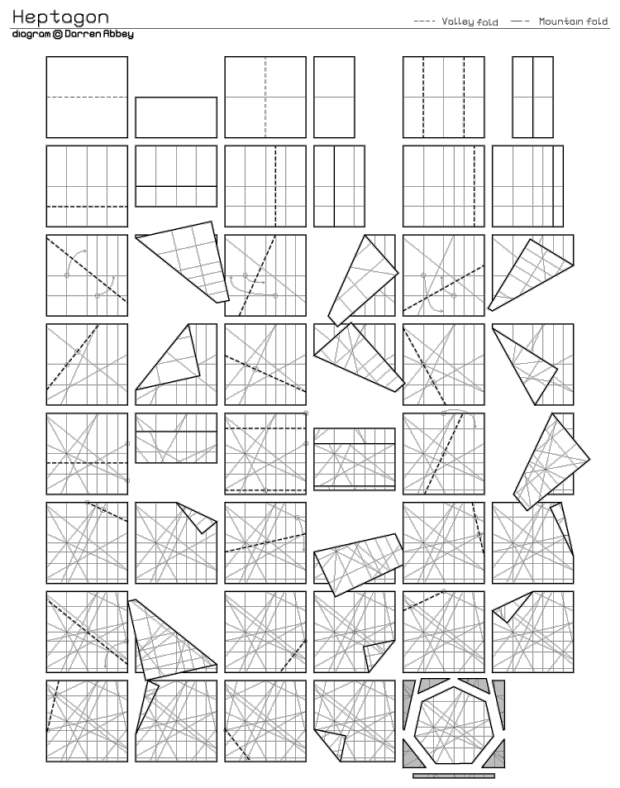
\includegraphics[scale=0.5]{7-gons.png}
    \caption{折纸正7边形}
\end{figure}